%!TEX root = ../../dissertation.tex
%%%%%%%%%%%%%%%%%%%%%%%%%%%%%%%%%%%%%%%%%%%%%%%%%%%%%%%%%%%%%%%%%%%%%%%%%%%%%%%%
\chapter{Reliable Video Streaming in Mobile Networks: Improving and Analyzing}
\label{chap:mobilestreaming}

The analyses of the previous chapter were entirely based on having access to mobile core network measurements. Most research groups will in most likelihood not have this access and have to rely on active end-to-end device measurements or other approaches.

Furthermore, the notion of the importance of reliable video streaming in mobile networks was also not picked up in the previous chapter. Both the measurements of mobile networks as well as reliable streaming were treated as entirely separate aspects up until now. But, as data from mobile Internet traffic analyses and forecasts suggests \cite{cisco2014VNI}, video is already occupying a large portion from mobile traffic and might rise to an even higher ratio in the near future.

This chapter aims to rectify this split of approaches with two further lines of discussions. 

First, the existing higher layer protocols of a mobile device's reliable video network stack and the influences of lower layer mobile layers on them are analyzed. This focuses especially on new and upcoming protocols and changes to existing ones. This also ties in with the mobile network load influencing factors discussed in Section~\ref{c4:loaddefinition}. Any behavior exhibited in the device's stick could also have positive or negative effects on the network's control plane and signaling procedures. The section concludes with a theoretic cross-layer information exchange model that has the potential to improve 

Second, now that the stack has been discussed fully, several approaches to monitor and measure end-to-end mobile network traffic, and video in particular, are demonstrated and executed. No access to in-network measurement probes limits the level of detail one can deduce from influence sources inside the network. But it also opens up a wide range of other device-based information sources, some of which are crucial in mobile devices, especially regarding mobility. These methods are also not limited to particular mobile network architectures and can thus be used to rapidly compare new architecture evolutions or specific core network implementations to each other. 

Finally, a full video streaming mobile network simulation model is also presented with some initial results.


%!TEX root = ../../dissertation.tex
%%%%%%%%%%%%%%%%%%%%%%%%%%%%%%%%%%%%%%%%%%%%%%%%%%%%%%%%%%%%%%%%%%%%%%%%%%%%%%%%
\section{Recent Developments in the Mobile Network Stack}
\label{c5:sec:stack-enhancements}


Contrary to the popular scientific belief, that the Internet is unable to change and renew itself (so called Internet ``ossification'', compare, e.g., \cite{feldmann2010ossification}), protocols in the \gls{TCP}/\gls{IP} stack change all the time. Changes are more likely to occur in the end-to-end stack behavior and not in the packet format, as they are more difficult to change. New application requirements and changing network architectures always trigger adaptations in the stack in-between. 

Superficially not much has changed, there is still \gls{IP}, \gls{TCP}, and \gls{HTTP} forming effectively the same protocol stack since 1991 with HTTP/0.9. And this seems hard to change, especially the transport layer is fixed to \gls{UDP} and \gls{TCP}, everything else will probably get rejected and dropped by one of the numerous middleboxes, such as \glspl{NAT} or firewalls.


In this section





%%%%%%%%%%%%%%%%%%%%%%%%%%%%%%%%%%%%%%%%%%%%%%%%%%%%%%%%%%%%%%%%%%%%%%%%%%%%%%%%
\subsection{Influences of the Existing Stack}

Improvements to congestion control for mobile streaming?


 Influence of L1/2/3 layer protocols and mechanisms (IPv4/6, tunneling, ethernet vs RLC/RRC/NAS, ...)


using TLS or not

Firefox Patch: Sort Idle HTTP Connections by CWND \cite{ffSortCWND}

%%
Bufferbloat, Congestion Control, and AQM Effects on Reliable Mobile Streaming

 ECN~\cite{rfc3168} (one of the earlier notions of cross-layer interactions; disabled by default almost everywhere)

Comparison of end-to-end and network-supported fast startup congestion control schemes \cite{scharf2011comparison}

Bufferbloat: Dark Buffers in the Internet \cite{gettys2011bufferbloat}

Detecting and quantifying bufferbloat in network paths \cite{groenewegen2011detecting}

Congestion avoidance and control \cite{jacobson1988congestion}

Controlling Queue Delay \cite{Nichols:2012:CQD:2209249.2209264} CoDel\cite{nichols2014codel}
 TCP needs congestion loss to determine bottleneck line speed
	too much buffering hinders this
 Memory is cheap, so why not put in some more megabytes
 Home router buffer induced latency can be as high as several seconds
CoDel:
 Head drop not tail drop
 Queues only as shock absorbers
 What matters is the delay within a flow
 CoDel measures minimal packet pass through time in the local device buffer during a defined interval
 If minimum gets too high, too much buffering is happening
 If delay value does not once fall below a target in the interval CoDel will start dropping packets
	Signals congestion and hopefully reduces source rate
	If stays above target, progressively more packets are dropped
	Target: 5ms; interval: 100ms, based on simulation results
 Can be enabled in Linux since 3.5, but many NIC drivers do not support it yet
 Every buffer along the path influences transmission
	Most impact on the node before the bottleneck
	Cell towers, dsl/cable modems, ...




Characteristics of UDP packet loss: Effect of tcp traffic \cite{sawashima97characteristics}


%%
Mobile Network Architectures, end-to-end Protocol Stacks and their sensitivity to Middleboxes



%%%%%%%%%%%%%%%%%%%%%%%%%%%%%%%%%%%%%%%%%%%%%%%%%%%%%%%%%%%%%%%%%%%%%%%%%%%%%%%%
\subsection{Upcoming Protocols and Streaming Relationship}


 Alternative modes of transport (e.g. DCCP, , RED, Google's SPDY or new approaches)

 Alternate Transport Protocols (DCCP\cite{rfc4340}, LEDBAT\cite{rfc6817}/$\mu$TP\cite{bt2010utp}, QUIC, SCTP~\cite{rfc4960}, DTLS~\cite{rfc6347})

but successful protocols develop de-facto; de jure much harder (see \gls{3G})



 End-to-end encryption and Authentication mechanisms (e.g.IPSec~\cite{rfc4301}, DNSSEC~\cite{rfc4033}, \gls{DANE}~\cite{rfc6698})


\gls{QUIC}  Quick UDP Internet Connections; protocols without retransmission feature (lost packets are not relevant and cause head-of-line blocking) but still with the all-important congestion control + TLS
%http://www.ietf.org/proceedings/88/slides/slides-88-tsvarea-10.pdf
\footnote{\url{http://lwn.net/Articles/558826/}}
UDP based for now, could very well end up as modifications to future TCP
inherits new TCP features such as TFO, snap start, ...
avoids most retransmissions through FEC
congestion control not through CWND but through packet pacing
includes stream multiplexing and TLS-like crypto by default



WebSocket \cite{rfc6455}
WebSockets as streaming transport \cite{w3c2011websockets} \cite{heise2011websockets}
 IETF HyBi (Hypertext Bidirectional) Working group
 W3C WebSocket API
 Supported by every major browser and Web server
 Provides full-duplex client-server communication
	Upgrades from HTTP/1.1 through extension header
	Barebone protocol atop TCP (or TLS), not HTTP
	HTTP/1.1 only allows client-initiated polling (GET)
	Asynchronous server push possible
		In HTTP/1.1 only achievable through various hacks (e.g. ``long polling'')
		Stateful instead of stateless (as HTTP)
Lower overhead per transmission/frame
Reduces number of open TCP connections and bandwidth overhead (no polling on additional TCP connection)


WebRTC \cite{webrtcdraft}


SPDY: An experimental protocol for a faster web \cite{google2011SPDYdef} and \cite{google2010SPDYwp} 
SPDY / \gls{HTTP}/2.0 (multiplexing -> segmented streaming)
 Google proposal and draft
	Currently SPDY/3.1 
	IETF httpbis working group basis for http/2.0
 original Draft based on Chrome browser implementation
 Widespread use and implementations
	Chrome, Firefox; Apache, Nginx
	Google, Twitter, Facebook, Akamai, Wordpress, ...
	HTTP-requests are transparently upgraded through Next Protocol Negotiation
 TLS mandatory
 HTTP/1.1 syntax still viable as a layer on top of SPDY
 Aim: Just one connection held per domain
	Better server scaling (less concurrent connections, fewer packets sent)
	Better latency
Multiplexing/Streams:
 Control and Data Frames, with header compression
 Stream interleaving/multiplexing or cancellation
 Server hint
	Server informs client, what he might want to request in the near future
 Server created streams / server push
	Avoiding one additional RTT and polling
	Only data pushed related to possible GET requests
	Client-side throttles to prevent ``push attacks''
 Stream priorities (8 levels)
	Prefer essential resources over others (images)
	Prefer data with earlier deadlines? (E.g. load next few video streams immediately while already requesting more)
 Use with Scalable Video Coding (Base Layer vs Enhancement Layers)?
 Per stream flow control
multiplexing:
 HTTP: One file request after another
	Pipelining usually absent or disabled by default in browsers (Chrome, Firefox, IE)
	High complexity/maintenance, low gain, head-of-line blocking issues
 SPDY: File parts reordered according to timelines
	Out of order and interleaved requests
Evaluations:
	Average reduction in page load time: ~29\%; 27\% - 60\%
	Strongly dependent on connection, server environment
	HTTP/1.1 optimization (resources split on multiple domains) prevents SPDY multiplexing gains
 SPDY could be more susceptible to packet loss and TCP congestion window downscaling
	Only one connection used compared to multiple HTTP/1.1
 Possible operator benefits
	Significant reduction in concurrent TCP sessions
	Reduction in packets per second
	$\rightarrow$ Reduced infrastructure load?
spdy mobile page load times
 Chrome on Android tests with several Websites
 Emulated mobile conditions (constant 2Mbps, 150ms RTT)
 ~23\% average load time reduction
 Benefits can be higher for large RTT
	Less request round trips and connection setups needed



HTTP/2.0~\cite{http20draft}
 HTTP/1.0 defined in 1996, 1.1 in 1999
	Since then no changes changes to the core protocol
 Many long standing issues with HTTP/1.1, e.g.
	Problems with ``long fat pipes''
		Many parallel connections as workaround
		Fairness issues
	Large overhead for small requests
 IETF Hypertext Transfer Protocol Bis Working Group
 Initial call for proposals made in March 2012
 Planned 2.0 standard proposal in 2014/2015
 Using SPDY as a starting point
 General aims
	Tackle multiplexing, improve load times and experienced latency
	But preserve the semantics of HTTP/1.1
requires presence (but not usage) of TLS1.2
	if used, emphemeral cipher suites >=2048 must be used (a.k.a. Perfect Forward Secrecy)












%%%%%%%%%%%%%%%%%%%%%%%%%%%%%%%%%%%%%%%%%%%%%%%%%%%%%%%%%%%%%%%%%%%%%%%%%%%%%%%%
\subsection{The TCP Case: Prime Example of a Living, Ever-Evolving Protocol}

\gls{TCP} changes (Fast Open, IW10, ...; any relationship to streaming? maybe faster)

TCP modifications for short-lived connections (e.g. initially ignore congestion avoidance and push a lot of data at once (google.com approach, Increasing TCP's Initial Window)) 

IW10: better response time, still fair \cite{rfc6928}
An argument for increasing \gls{TCP}'s initial congestion window \cite{dukkipati2010argument}
IW3, IW10  Initial window size (IW10, ...)
 TCP Congestion Window
	Maximal number of packets in flight
–	Scaling through congestion control and avoidance algorithms
 Initial Value
	1 (RFC1122, RFC2001)
	4000 Bytes (~ 3 packets) (RFC2414, RFC3390, ~2002)
	IETF proposal: IW10 (Google Draft 2010-2012)
 Rationale
	HTTP request for small websites using new TCP connection
	Transmit whole site in one RTT instead of multiple
	Reduces average latency
		Evaluation: ~10\% page load reduction on typical web pages
	High IW values already used by many CDNs



TCP Fast Open~\cite{cheng2014tcptfo}
 IETF draft
 Linux 3.6 client side implementation (September 2012)
 Linux 3.7 server side (~ 2012)
 Small server-side application adaptation required
 Send data in the SYN and SYNACK packets
	Deliver it immediately to the application
	Only allowed for subsequent connections, requires additional security cookie (specific to client-server IP pair)
 Saves one initial RTT
 4\% to 41\% popular web page load time improvement


1s / 3s Retransmission Timeout \cite{rfc6298}
 TCP retransmission timeout set through RTT measurement
 Default value needed for timeouts during handshake: 3 seconds (now obsolete RFC1122, RFC2988)
 RFC 6298, Linux 3.1 (October 2011)
	Reduce TCP initial retransmission timeout to 1 second
 Improves TCP handshake times for lossy networks
 Benefits for short-lived (Web) transactions


Proportional Rate Reduction PRR (vs. rfc 3517)
 TCP behavior on packet loss in the past
	RFC 3517: reduce CWND to half
		Must first ACK large portion of the data still in flight before transmitting again
	Linux: ``Rate halving''; Reduce CWND by 1 on every ACK until CWND/2
		Can still send data during recovery
 Google IETF Proposal (Linux 3.2, January 2012): PRR
	Reduce timeouts by avoiding excessive window reductions
	Converge to cwnd chosen by congestion control by the end of recovery
	Can improve packet loss recovery time and average latency



TCP Early Retransmit \cite{rfc5827} Kernel 3.5 (July 2012)
 TCP loss recovery (not using SACK) triggers on
	Timeout (may be lengthy, ~RTT, min 1s)
	Triple duplicate ACK (fast retransmit)
		If CWND is small, TCP may not be able to get enough DUPACKs to trigger
		Reduce DUPACK threshold for these connections
 Reduce DUPACK threshold for these connections
	Less robust to segment reordering
 Reduces average latency for narrow and lossy connections

Multipath TCP MPTCP~\cite{rfc6824}!


Congestion Avoidance algorithm ((New Reno~\cite{rfc6582}, Vegas~\cite{Brakmo:1994:TVN:190809.190317}, Compound~\cite{song2006compound}, BIC, CUBIC~\cite{ha2008cubic}; all w or w/o SACK)
general basic tcp congestion control in \cite{rfc5681}, describing Reno

Slow Start~\cite{rfc5681}
 HyStart~\cite{Ha20112092}


Nagle's Algorithm~\cite{rfc896} delaying and aggregating small data packets


OS-dependent receive window scaling behavior

OS-dependent choice of packet size


%%%%%%%%%%%%%%%%%%%%%%%%%%%%%%%%%%%%%%%%%%%%%%%%%%%%%%%%%%%%%%%%%%%%%%%%%%%%%%%%
\subsection{Proposal for Cross-Layer Enhancements}
\label{c5:crosslayerhinting}


Wired Internet access has a very narrow choice of protocols on the \gls{ISO}/\gls{OSI} Layers 1 and 2. The typical use-case consists of a \gls{LAN} using Ethernet which is then tunneled through or translated into one of several access technologies, e.g., \gls{DSL}, \gls{DOCSIS}, or \gls{PON}. Applications often make assumptions that rely on the presence of these protocols and their specific characteristics.

However, Internet access today is similarly often achieved using mobile cellular networks. The latest standardized iteration of these is \gls{LTE} and the accompanying \gls{EPS} core network infrastructure \cite{olsson2009sae}. This is the first evolution of standards that completely removes the classical circuit switched domain making room for more radio frequency bandwidth to be used with the all-\gls{IP} services achieving shared transmission capacities --- comparable to today's 802.11n WiFi --- albeit on much larger cell sizes of \SI{1}{\kilo\meter} to \SI{3}{\kilo\meter}. The \gls{EPS} network acts as an intermediary between the radio access stations and the Internet enabling strong traffic control mechanisms as well as mobility anchored at the \gls{SGW}. Traffic is routed through the core by using tunneling over the \gls{SGW} and \gls{PGW} based on the traffic bearer concept defined either in the \gls{gtp} or the \gls{PMIPv6} protocols. For every mobile device connected to the network there is one default and up to ten dedicated bearers carrying traffic filtered by pre-set \gls{QoS} parameters. Control is enforced through a logically separate network control plane, that is also used to setup and tear down these bearers. Figure fig:ltestack displays the disparity between the Internet's protocol stack and that of an \gls{LTE} network encapsulating all user traffic in additional protocol layers by the tunneling process.

Research work is ongoing how to best work with this complex network setup. It is expected, that with the rise of mobile access the core network comes under heavy traffic pressure with negative affects on the \gls{QoS} of best-effort traffic. Endeavors are required to study the loaded network's behavior. Also very little work has gone into exploring the control plane characteristics of these networks, including their performance. A novel approach could also be, to make mobile device applications, e.g. video streaming players, aware of the core networks capabilities and allow the request of tunnels tailored to their specific \gls{QoS} requirements resulting in a possible increase of perceived quality.

% influence of signaling plane and core network elements - scaling

The protocols used for the radio transmissions behave very differently when compared to Ethernet and assumptions made by higher layers may not hold any more. This can apply to, e.g., reliability, frame sizing and fragmenting, and latency amounting to undesired effects on higher-layer traffic. For example, loss in \gls{GSM} and \gls{UMTS} networks is often caught transparently on layer 2 and a retransmission is conducted. However, in the time the retransmission takes the transport layer may have already run into a timeout and re-requested the missing segment on its own, resulting in additional delay and a waste of bandwidth. This is especially detrimental for time-critical applications like video streaming, possibly resulting in buffer underruns and degraded quality. Transport and application layer mechanisms need to be able to understand this and cope with the effects. E.g., \gls{TCP} retransmissions and congestion control could be adjusted in the course of understanding this.

Furthermore, traffic could be avoided during cell handover occurrences. This would require cross-layer cooperation and an awareness of the application when an handover is supposed to occur. The application then could schedule its traffic accordingly. Traffic falling into a handover is subject to especially high latency and loss because the mobile network acts as a mobility anchor which needs to internally reroute incoming traffic to the mobile device's new position. \gls{HTTP} traffic is especially suited to this scheduling behavior because of its statelessness and consistence of small objects that can be requested and transferred independently.


\subsubsection{Related Work}

\begin{itemize}
	\item Cross-layer design optimizations in wireless protocol stacks \cite{Raisinghani2004720}
	\item ECLAIR: An efficient cross layer architecture for wireless protocol stacks \cite{raisinghani2004eclair}
	\item Still no implementation of ECLAIR: ``Cross-layer feedback architecture for mobile device protocol stacks'' \cite{1580937}
	\item 802.21
	\item A multi-layer mobility management architecture using cross-layer signalling interactions\cite{wang2003multi}
	\item 
		\begin{itemize}
			\item \gls{DLEP} \cite{ietf2013dlepdraft}
			\item running on routers for communication between routers and attached interfaces (wireless!)
			\item interface/modem informs router about link characteristics
			\item router acts upon this information
			\item specific set of required and optional signals (message types / reason for messaging) and data items (information)
			\item bandwidth, latency, connection status (loss)
			\item information about specific neighbors
			\item \gls{UDP}-based, discovery mechanism via multicast, session-based
			\item requires/relies on lower layer auth/crypt
			\item no data items specific for cell-type mobile nets and mobility
			\item best suited for routers with external modems/interfaces (outside antennas)
		\end{itemize}
	\item Seamless Mobility in Heterogeneous Wireless Networks \cite{zarai2010seamless}
	\item Radio resource management in emerging heterogeneous wireless networks \cite{Piamrat20111066}
	\item Improved community network node design using a DLEP based radio-to-router interface \cite{6379143}
	\item Cross-layer signalling for next-generation wireless systems \cite{1200522}
	\item Cross-layer design for wireless networks \cite{1235598}
	\item A cautionary perspective on cross-layer design \cite{1404568}
	\item User-centric mobility management for multimedia content access \cite{bolla2011usercentric}
	\item Socketless \gls{TCP} --- an end to end handover solution \cite{1635680}
	\item SATSIX cross-layer architecture \cite{4656786}
	\item mostly routing protocol optimization oriented ``A cross layer based QoS model for wireless and mobile ad hoc networks'' \cite{krishna2007cross}
	\item SmoothIT mechanisms; lower layer elements provide information to higher layers, overlays\footnote{\url{http://www.smoothit.org}}  \cite{oechsner2009pushing}
	\item ``Mobility Awareness'' \cite{hummel2010mobilitaet} PMLAR (Predictive mobility and location-aware routing protocol in mobile ad hoc networks)
	\item Automatic Multi-interface Management Through Profile Handling \cite{Bonnin:2009:AMM:1503496.1503498}
	\item A ubiquitous mobile communication architecture for next-generation heterogeneous wireless systems \cite{1452832} (supposed to propose a function that determines the best handover initiation time in order to avoid early or late initiations)
	\item Optimized video streaming over 802.11 by cross-layer signaling \cite{1580941}
	\item LCP Link Control Protocol, PPP extension RFCs \cite{rfc1570,rfc1661}
 	\item Modem Link Properties Advertisement Protocol\footnote{\url{https://tools.ietf.org/html/draft-ivancic-mobopts-modemlpa-01}}
	\item IEEE 802.21 cooperative handovers, but with required network support
	\item LISP and other mobility approaches \cite{rfc6830}
	\item Radio Resource Management RRM
		\begin{itemize}
			\item resource monitoring, decision making, decision enforcement
			\item choose available wireless interfaces  best suited for a specific task
			\item rudimentary implementations in mobile OSs
		\end{itemize}
\end{itemize}




%%
\subsubsection{Cross-Layer Mobility Hinting}

Today's mobile networks are all of a cellular design. A device that moves from one cell to the other has to perform a so-called handover. During this process the device is deregistered in one cell and registered in the new one. All network traffic currently in flight has to be rerouted or relayed to the device's new location. 
Although seemingly transparent to the device's application, adverse side effects can occur during a handover, including an increase and variability of latency. 

Mobility support today always means network assisted mobility. Typically, the network decides the best possible mobility strategy from its point of view and provides infrastructure to support seamless handovers in the form of mobility anchor nodes. However, the device is actually in a very unique position, as it knows a great deal more about its traffic mix, its currently running applications and its user than the network ever could and should.
Unfortunately, most of this information remains unused, as today's network infrastructures and lower layer protocol stacks provide only very slim changes to exert control over decisions regarding the device.

Nonetheless, a lot could still be done when providing the device's operating system and application ecosystem with a simple bidirectional pathway for vertical information and control flow across network protocol layers and to other low-level systems. This work aims to do just that by providing a generic interface and exchange protocol for any kind of information relevant to an application's decision making process. With this meaningful actions and reactions of individual layers can be defined and tested. Possible use cases are provided in the next section.

Still, one has also to keep in mind, that layering and encapsulation is there for a reason and violating this is a rather risky undertaking. However, we do not think that our approach actually violates these basic principles and only extends on the ways one can communicate and interact with all individual layers without changing anything in them.


	% - Research objectives
	% 	- Bidirectional vertical information and control flow on the performance of the individual layers
	% 		- Definition of generic interfaces
	% 		- Definition of a protocol (including information types, etc.)
	% 	- Definition of meaningful actions/reactions on the individual layers (e.g. adaptation of real-time communication data sources or changes in resource allocation)

		

\subsubsection{Scenario Use Cases}

\begin{itemize}
	\item Video/Voice calls that notify the other party, that interruptions are expected to occur.

	\item Using current location data and movement patterns/predictions to improve cell selections and initiate horizontal and vertical handovers to a time suitable for the device and running applications.

	\begin{figure}[htb]
	        \centering
	        \begin{subfigure}[b]{0.90\textwidth}
	            \centering
				\includegraphics[width=\textwidth]{images/adaptive-streaming-no-cl.pdf}
				\caption{Stalling occurs without handover hinting.}
				\label{c5:fig:streaming-hinting-no-cl}
	        \end{subfigure}%

	        \begin{subfigure}[b]{0.90\textwidth}
				\centering
				\includegraphics[width=\textwidth]{images/adaptive-streaming-cl.pdf}
				\caption{Stalling can be prevented by hinting and proactively filling the playback buffer.}
				\label{c5:fig:streaming-hinting-cl}
			   \end{subfigure}%
	 \caption{Mockup of handover prediction and hinting for adaptive streaming and thus avoiding playback stalls.}
	\label{c5:fig:streaming-hinting}
	\end{figure}

	\item An adaptive streaming video application increases its video buffer when a shortly upcoming handover is announced to survive the service outage. This can be achieved by an increased rate of segment retrieval and a reduction in segment quality. The goal is to avoid any possible playback stalls due to the handover. Figure~\ref{c5:fig:streaming-hinting} demonstrates this circumstance.

	\begin{figure}[htb]
	        \centering
	        \begin{subfigure}[b]{0.90\textwidth}
	            \centering
				\includegraphics[width=\textwidth]{images/http-reorder-no-cl.pdf}
				\caption{The handover will block currently active object transmissions, page display will be delayed.}
				\label{c5:fig:http-reorder-no-cl}
	        \end{subfigure}%

	        \begin{subfigure}[b]{0.90\textwidth}
				\centering
				\includegraphics[width=\textwidth]{images/http-reorder-cl.pdf}
				\caption{The browser reorders the objects to be retrieved and avoids any transmissions during the indicated handover period.}
				\label{c5:fig:http-reorder-cl}
			   \end{subfigure}%
	 \caption{Mock-up of \gls{HTTP} reordering with handover awareness.}
	\label{c5:fig:http-reorder}
	\end{figure}

	\item Enable applications to adapt themselves to the conditions currently experienced by the networking stack and its sensors. For example, a Web browser could reorder its Website object requests to avoid sending any requests during handover periods and experience additional delay as seen in Figure~\ref{c5:fig:http-reorder}.

	\item A cross-layer enabled device can also offer a wide range of policy choices to its applications or even directly to the user. An example rule could be: ``Do not handover to a stationary WiFi from 3G when moving faster than 50km/h, only to in-vehicle WiFi.'' or ``Avoid any vertical handover, which would interrupt my service for a long time, while this VoIP call is running.''

\end{itemize}

\subsubsection{Technical Implementation}

The Implementation:
\begin{itemize}
	\item Userspace daemon that collects information from kernelspace protocol implementations and sensors and provides them to all applications.
	\item shared bus control/information system, instead of explicit comm; signaling only to interested parties
	\item provide common interface also to all available sensors and layer 1 and 2 network information and control (similar to Android)
	\item IPC message bus, possibly D-Bus\footnote{\url{http://www.freedesktop.org/wiki/Software/dbus/}} based
	\item Could extend NetworkManager\footnote{\url{https://wiki.gnome.org/Projects/NetworkManager}}, some functionality is already provided there

\end{itemize}

The process:
\begin{itemize}
\item Tell Transport/Application the expected time till handover / time of uninterrupted service
\item Tell Transport/App expected connection parameters (latency, BW, ...)
\item Application selects \gls{DASH} stream appropriate to parameters
\item Application reorders \gls{HTTP} GETs so that large GETs are not interrupted
\item Application stops transfers when handover is about to occur
\item Layer 1/2 gives a list of possible handovers to Application
\item Application selects (better: suggests) handover which fits best and reorders accordingly
\end{itemize}


\subsubsection{Planned Work and Methodology}

\begin{itemize}
	\item investigate how much information is exposed and what can already be done
	\item Analysis of data traces and realistic simulations in order to capture in detail the unwanted phenomena
	\item Verify the suitability of the State-of-the-Art algorithms and protocols which address this problem
\end{itemize}


%!TEX root = ../../dissertation.tex
%%%%%%%%%%%%%%%%%%%%%%%%%%%%%%%%%%%%%%%%%%%%%%%%%%%%%%%%%%%%%%%%%%%%%%%%%%%%%%%%
\section{Measurements}
\label{c3:measurements}

With these playback models at hand, this section demonstrates how to conduct actual evaluations of reliable streaming protocols with it.

As discussed, there are numerous incarnations of reliable streaming protocols in use. Almost all of them follow the same basic approach but with slight variations in execution and choice of playback strategies and corresponding parameters. But it is exactly these choices that can have a large impact on the streaming process and resulting quality. 

The problem lies in comparing these protocols to each other. Each of them is usually tied to a specific -- and most often proprietary closed source -- streaming player. Setting up all these players in one testbed is a huge effort and requires very specific software environments to be used on the client machines. Moreover, these players are built with user interaction and not automation and directly measuring the outcome in mind. This can still be achieved through extensive workarounds, but must be tailored to every player application. The presented approach avoids this hassle and provides a concise way to test any conceivable playback strategy in one single test setup.


%%
\subsection{Progressive Streaming Measurement Framework}

To enable quick evaluations for progressive streaming the framework follows a two phase approach, separating the active online recording phase from the passive playback emulation. Recording data is very time intensive and cannot be sped up when conducting investigation of a real world process, and not relying on simulated data. It still replicates the steps a user would perform to consume a media stream on a playback device. Through appropriate configuration different scenarios can be modeled, e.g. network conditions, behavior and specifics of the user device.
 
\begin{figure}[htb]
    \includegraphics[width=\textwidth]{images/measurement-model.pdf}
    \caption{Measurement framework for progressive streaming playback strategies overview.}
    \label{c3:fig:framework}
\end{figure}

Figure \ref{c3:fig:framework} depicts the framework for a streaming evaluation testbed. In phase one the stream's transmission is conducted and recorded on a per-packet level. Stream data is transmitted to the client from a server which can be any actual streaming service on the Internet or a local server under the testbed's control, eliminating undesired side effects caused by the Internet connection. 

The traffic is directed through a network emulation node capable of altering the network \gls{QoS} parameters, i.e. latency, jitter, and packet loss. The parameters can be set according to stochastic models derived from actual network architectures. Instead of network emulation, any preexisting architecture can also be placed here to achieve more accurate results for the intended target. This is especially helpful for complex infrastructures hard to model or with no good and concise models available yet, for example mobile and mobile core networks with the influence of encapsulating traffic into bearers.

The measurement host downloads and records the video stream as a network trace. For progressive \gls{HTTP} streaming, a single request on the video file is issued and the \gls{TCP} connection maintained until the file has fully arrived.
This process is recorded as basis for the second phase. These traces should consist of the size and timestamp of every incoming packet. More detailed traces can be used to scrutinize other layers of the connection, e.g. the dynamics of TCP receive window size. Additionally the received file is decoded yielding a trace of all video frame sizes and playout timestamps.

In the second pass, these two traces are then used to feed the actual reliable streaming playback model described before. This conducted by a closed-loop emulation process calculating the current buffer fill level based on the collected transmission and video frame traces for every point in time. 

All of the progressive streaming -- i.e. non-adaptive -- strategies can be tested on the same trace set.
In simple \gls{HTTP} streaming, the transmission is not controlled by the streaming application and no rate control is conducted. Therefore, recording the packet trace and simulating playback are completely decoupled, as the latter cannot influence the former.  This enables fast and efficient comparison of non-feedback protocols subject to the same network conditions.

The emulator then generates playback stalling statistics, specifically their number and duration, to compare the effect of the different strategies on the same trace. With these results, parameter settings for playback strategies can also be iteratively tested and improved leading to an empirical calibration of playback strategies instead of relying on best practices.

One of the drawbacks of this model-based emulation approach is of course the reliance on suitable models and playback strategies for the stream protocols under scrutiny. Obtaining these from proprietary streaming clients, can be a difficult reverse-engineering process.


%%
\subsection{Adaptive Streaming Measurement Framework}

Up to this point, the measurement framework is only suitable for progressive streaming omitting any adaptive strategy. This second framework modifies this and additionally allows for the testing of adaptive playback strategies. However, to achieve this, the advantageous two phase setup cannot be employed anymore.

\begin{figure}[htb]
    \includegraphics[width=\textwidth]{images/feedback-measurement-model.pdf}
    \caption{Measurement framework for adaptive streaming playback strategies overview.}
    \label{c3:fig:framework-feedback}
\end{figure}

Figure~\ref{c3:fig:framework-feedback} shows the adapted framework. The playback emulation process is now directly fed with the stream transmission without recording it first. The emulation is now an online process and has to be conducted in realtime. This enables the emulator to react on the current streaming state and request an alteration from the server. The adaptation spectrum ranges from the timing of stream segment retrieval to the chosen quality level of future segments. 

While allow for a wider range of playback strategies, this approach is also inherently slower as it does not allow a speed-up beyond realtime, limiting its usability somewhat. Therefore, a transition to a full simulative approach is suggested. This is path is further explored and discussed in Section~\ref{c5:mobilestreamingtestbed}.

\todo{check simulation approach ref or further explain simulation}


%%
\subsection{Technical Implementation}

To conduct measurements, the described two phase progressive streaming measurement framework was implemented in a testbed. This testbed consists of three interconnected physical nodes running Linux. 

The optional streaming server houses an Apache httpd\footnote{\url{https://httpd.apache.org/}} Web server, hosting the files that are to be streamed. Alternatively, Internet streaming service traffic can also be directly routed through the network emulation node.

The network emulation node uses the existing \gls{QoS} capabilities of the Linux kernel, dubbed NetEm \cite{hemminger2005network}, to add latency and packet loss to the transmission as well as to act as a bandwidth bottleneck. The additional delay is set deterministically, the loss follows a uniform distribution without any correlation in the transmission.

To both retrieve the streaming file and record the transmission process at the client, curl\footnote{\url{http://curl.haxx.se/}} is used. If so desired, tcpdump\footnote{\url{http://www.tcpdump.org/}} can also be facilitated to achieve a higher recording precision. The video file is then parsed for its frames and sizes using mplayer\footnote{\url{http://www.mplayerhq.hu/}} with libav\footnote{\url{https://libav.org/}}. The traces are then put into the actual playback emulation, implemented by custom Python-based code and statistically evaluated with Python as well as R.



%%
\subsection{Measurement Series and Evaluations with the Framework}
%[visualization and results (does yt still work well with high delay/loss?)]
%[performance evaluation (BWs, played vs received data)]
%Also observed and analyzed. The deduce that the initial buffering time and the later block sending rate are directly correlated. 64kb blocks, probably due to GFS, problems with this method, ...
%These Quality-of-Service parameters loss and delay do not have any direct influence on the downloading process but instead have negative impacts on the throughput of the underlying TCP due to its congestion control feature and, in the end, serve as another source of delay and jitter.

This implementation has been used to conduct a comparative study of two theoretical and two real world playback strategies. They are tested for their susceptibility to worsening network \gls{QoS}, latency and loss in this case.

The video used in the experiment was streamed from the YouTube web site providing a realistic foundation for the experiments. This also enables a server side pacing mechanism adjusted to the video bitrate for free
Details on the video used in the experiment are available in Table~\ref{c3:tbl:videoparams}. Two measurement series are performed with this video, both only differ in the network emulator setting. The first series increasingly adds packet loss to the stream, with the second series altering the packet delay. 

\begin{table}[htbp]
    \centering
    \caption{Test Video Parameters}
    \label{c3:tbl:videoparams}
    \begin{tabu}{|l|X[r]|}
        \hline
        Parameter & Value \\ \hline
        Video Duration  & \SI{92.536}{\second}\\
        Size & \SI{9.61}{\mebi\byte} \\
        Framerate & \SI{23.976}{\per\second} \\
        Average Video Bitrate & \SI{871}{\kilo\bit\per\second} \\
        Codecs & AVC+AAC \\ \hline
    \end{tabu}
\end{table}


%% latency
In the latency measurement series, the emulator delayed forwarding the packets for a constant amount of time
The latency was increased in \SI{100}{\milli\second} steps, up to a total of \SI{5000}{\milli\second}. The added latency is split up evenly between the uplink and the downlink.


It can be stated, that all playback strategies will generally work very similar under good network conditions. If sufficient bandwidth is available, they will play videos with almost no delay or intermediate buffering. 
If, however, the achievable \gls{TCP} goodput is close to the average video bitrate, the buffer can be quickly drained by short deviations from the average transmission and video bit rates. The \gls{TCP} goodput can be limited by high latency and loss. Many \gls{TCP} congestion control algorithms depend on the round trip time. If the \gls{RTT} is high, the congestion window will increase much slower. High latency can also trigger \gls{TCP} timeouts and retransmissions, and in turn decrease the congestion window, further impacting the goodput. 

%% <-- WIP

The latency measurements are depicted in Figures \ref{c3:fig:eval-latency-stallingtime} and \ref{c3:fig:eval-latency-numstalls}. The stalling time increases with the additional latency. The Initial Start Delay model provides the best possible result in terms of pure stalling time. On the other hand, Figure \ref{c3:fig:eval-latency-numstalls} shows the Stalling model provides always the worst result for the number of stalls. Any other model will lie beyond that line. The Flash and HTML5 models both run in just a few buffering events which however tend to increase in length with rising latency. Attributed to the simple and optimistic assumption of the Flash model, stalling time is usually lower than with HTML5, at the cost of slightly more buffering events.
 

\begin{figure}[htb]
    \centering
    \includegraphics[width=\textwidth]{images/eval-latency-stallingtime.pdf}
    \caption{Total stalling time.}
    \label{c3:fig:eval-latency-stallingtime}
\end{figure}

\begin{figure}[htb]
    \centering
    \includegraphics[width=\textwidth]{images/eval-latency-frequency.pdf}
    \caption{Playback model observations on additional latency. Number of stalls.}
    \label{c3:fig:eval-latency-numstalls}
\end{figure}


% loss
In the loss experiment series, uncorrelated uniformly distributed loss was added in both the uplink and the downlink direction. The loss was increased in $2\%$ steps up to a total additional loss of $14\%$

TCP goodput is even more severely affected by packet loss. A lost packet results in a duplicate acknowledgement, retransmissions, and a decrease of the congestion window. The problem gets worse if also the ACKs are lost and the connection stalls on missing old segments without which the playback cannot proceed. Figure xyz shows some exemplary measurements for a loss scenario. While additional packet losses of up to four percent seem to have no noticeable impact on streaming quality, the total stalling time suffers a large increase for any model as seen in Fig. \ref{c3:fig:eval-loss-stallingtime} rendering any streaming attempts practically unusable. Figure \ref{c3:fig:eval-loss-numstalls} shows the extremity of the Stalling model compared to other models reaching a number orders of magnitude larger than any other model.
As a result, when planning a network for streaming applications, the maximum loss should be kept below the noticed mark to achieve reasonable streaming quality. 


\begin{figure}[htb]
% used yt-delay/hPUGNCIozp0_delay_100 2, spyder with matplotlib config patch
    \centering
    \includegraphics[width=\textwidth]{images/eval-loss4mb-stallingtime.pdf}
    \caption{Playback model observations on additional packet loss. Total stalling time.}
    \label{c3:fig:eval-loss-stallingtime}
\end{figure}

\begin{figure}[htb]
    \centering
    \includegraphics[width=\textwidth]{images/eval-loss4mb-frequency.pdf}
    \caption{Playback model observations on additional packet loss. Number of stalls.}
    \label{c3:fig:eval-loss-numstalls}
\end{figure}
 
 %%




For this the simple stalling model is used because this results in the shortest possible playback duration in every scenario. Furthermore, we used a network emulation testbed to subject the video streaming to increased loss and latency while fixing the maximum network bandwidth and observe the influence on the QoE.

First use case to show how our system works: Progressive HTTP streaming. Will show adaptability to adaptive streaming and different protocols. For this comparison we used a video of about \SI{90}{second} length and network conditions that could not fulfill the video bitrate in time and hereby forced stalling to occur.

We performed two measurement series, one with increased packet loss, the other one adding latency to the path. For each value of loss and latency a mean total stalling time was calculated out of five separate experiments to eliminate temporal and network load influences. Additionally, standard deviations are shown in the resulting graphs. We clearly notice very large deviations in some experiments. Some of these can be explained by connection timeouts and later resumption of the streaming. Furthermore, an exponential regression line shows the trend of the total stalling times in the experiments.




%% <-- %% end WIP

\begin{figure}[htbp]
    \centering
    \includegraphics[width=\textwidth]{images/R-delayseries.pdf}
    \caption{Total buffering time and linear smooth for degraded network parameter scenarios. Latency Graph.}
    \label{c3:fig:delayseries}
\end{figure}

\begin{figure}[htbp]
    \centering
    \includegraphics[width=\textwidth]{images/R-lossseries.pdf}
    \caption{Total buffering time and linear model for degraded network parameter scenarios. Loss Graph.}
    \label{c3:fig:lossseries}
\end{figure}

Figure \ref{c3:fig:delayseries} displays the results of of the latency measurement series with up to five seconds of additional delay. In the worst case the stalling time increases to about 50 seconds. In mobile scenarios latencies of up to 2 seconds can be expected, which would, according to our measurements, result in a maximum mean stalling time of 15 seconds for a 90 second video, which could very well be bearable for YouTube users.

There are several factors that could contribute to the increase in stalling time in the latency experiments. 
TCP, in its simplest form, increases the congestion window based on the Round Trip Time (RTT), making it highly dependent on this connection parameter. Newer congestion avoidance algorithms, e.g. the CUBIC algorithm used in Linux \cite{ha2008cubic}, however reduce this dependence on the RTT.
Another influencing factor might be YouTube's block sending mechanism, which, according to \cite{alcock2011afcyt}, may negatively interact with congestion control algorithms. The impact of packet loss on stalling is much higher than that of latency in our measurements. Yet, due to TCP's reliable transmissions, loss only causes increased packet retransmissions, and, thus, acts as a source of burst delay which negatively impacts the overall throughput.

Figure \ref{c3:fig:lossseries} shows the series of loss experiments. While the 6\% packet loss and below has an almost negligible influence on the stalling time anything above this value will probably not achieve good user experience at all. Interesting to note is the rather sudden increase in stalling time when there is more than 6\% loss added. This could again hints to the transport protocol's reliable transport feature, which catches all the occurring losses, through timeouts or gaps in the sequence numbers. However, the detection and retransmission takes some time, which is reflected in the increased stalling time.







Through these to exemplary experiments, we tried to show that network QoS parameters have a direct measurable impact on the application layer, namely on HTTP streaming quality. While the models scale rather well with latency, any HTTP streaming is almost impossible with high packet loss values.
Comparing the presented playback models, we conclude that every model represents a trade-off between several parameters, e.g. as measured here, the number and length of stalls. With the knowledge gained from the experiments, playback models could be tailor-made to best suit certain conditions and user requirements. 




\section{Chapter Conclusions}



